%%*****************************************************************************
%% $Id: section-ide-eclipse.tex,v 1.3 2006/01/14 16:12:13 gene Exp $
%%*****************************************************************************
%% @author Gerd Neugebauer
%% @author Michael Niedermair
%%-----------------------------------------------------------------------------
\section{Eclipse}

Eclipse is a free IDE for Java and other programming languages. It
also provides a framework for the development of own programs. But
this is not needed for the \ExTeX\ core. Currently the version 3.1 of
Eclipse is used within the \ExTeX\ development team.
\begin{figure}[h]
  \centering  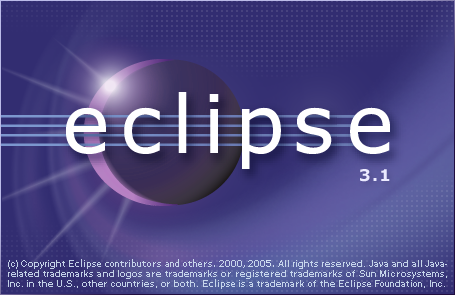
\includegraphics[scale=.5]{image/eclipse-splash}
  \caption{Eclipse}\label{fig:eclipse}
\end{figure}

\subsection{Eclipse Installation}

Eclipse can be downloaded for free from \url{http://www.eclipse.org}.
There you can get a file appropriate for your operating system
containing the software development kit (SDK). For instance
\begin{description}
\item [eclipse-SDK-3.1-win32.zip]\ \\
  for any decent Windows platform.
\item [eclipse-SDK-3.1-linux-gtk.zip]\ \\
  for Linux on Intel x86 with GTK.
\end{description}

Download the appropriate file and unpack it in the installation
directory. A new subdirectory \texttt{eclipse} will be created
containing all files of Eclipse. You are done with the basic
installation. You can start the \texttt{eclipse} executable found in
the just installed directory.

\begin{figure}[h]
  \centering  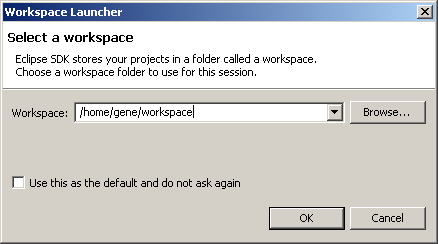
\includegraphics[scale=.5]{image/eclipse-workspace}
  \caption{Eclipse Workspace}\label{fig:eclipse-workspace}
\end{figure}
When Eclipse starts you first see the splash screen shown in
figure~\ref{fig:eclipse}. Then Eclipse requests a workspace -- as
shown in figure~\ref{fig:eclipse-workspace}. The workspace is a
directory where the projects live and where your preferences are
stored. If you have chosen the workspace directory carefully, you can
turn on the check mark in this dialog to be not asked again.

Finally you end up in the welcome window of Eclipse shown in
figure~\ref{fig:eclipse-welcome}. Take some time and read the
introductory material found there.
\begin{figure}[h]
  \centering  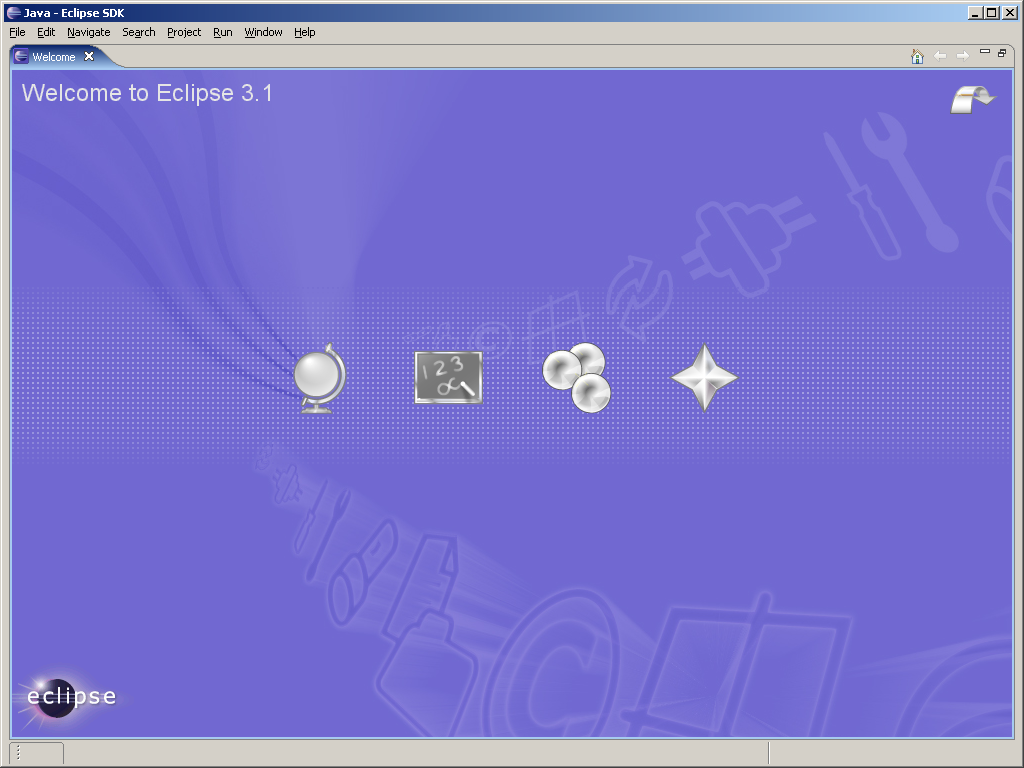
\includegraphics[scale=.33]{image/eclipse-welcome}
  \caption{Eclipse Initial Window}\label{fig:eclipse-welcome}
\end{figure}

The following sections describe some of the configurations which
should be performed in order to work with Eclipse on \ExTeX.


\subsection{Downloading the Sources}

Now we are ready to create a project for the sources of \ExTeX.
Everything needed can be found in the CVs repository of \ExTeX\ hosted
by Berlios.. Thus we start to get things onto the local host. For this
purpose we need to open a new perspective in Eclipse. A perspective is
a collection of windows which are usually meant for a common task.

A new perspective can be opened via the window \menu{Window \sub Open
  Perspective \sub Other\ldots} which can be seen in
figure~\ref{fig:eclipse-open-perspective-menu}. This menu item opens a
dialog box which offers some perspectives for opening. Currently we
need a ``CVS Exploring'' perspective. This perspective is meant for
inspecting CVS repositories and manipulation. Thus this perspective is
selected (see figure~\ref{fig:eclipse-select-cvs}) and the dialog is
completed with the OK button.
\begin{figure}[ht]
  \hbox{}\hfill
  \subfigure[Open Perspective\label{fig:eclipse-open-perspective-menu}]{%
    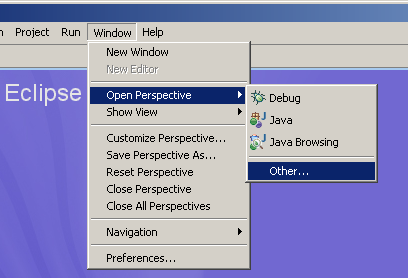
\includegraphics[scale=.4]{image/eclipse-open-perspective-menu}}%
  \hfill
  \subfigure[Selecting ``CVS Exploring Perspective''\label{fig:eclipse-select-cvs}]{%
    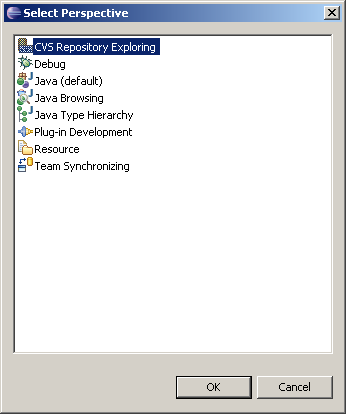
\includegraphics[scale=.4]{image/eclipse-select-cvs}}%
  \hfill\hbox{}

  \caption{Switching to a Perspective}\label{fig:eclipse-perspective}
\end{figure}

Now a CVS exploring perspective is opened (see
figure~\ref{fig:eclipse-cvs-1}). You see a lot of windows and icons
there. The tab ``CVS Repositories'' on the left side shows all
repository locations currently known. This list is empty since we have
not added any CVS locations yet.
\begin{figure}[htbp]
  \centering  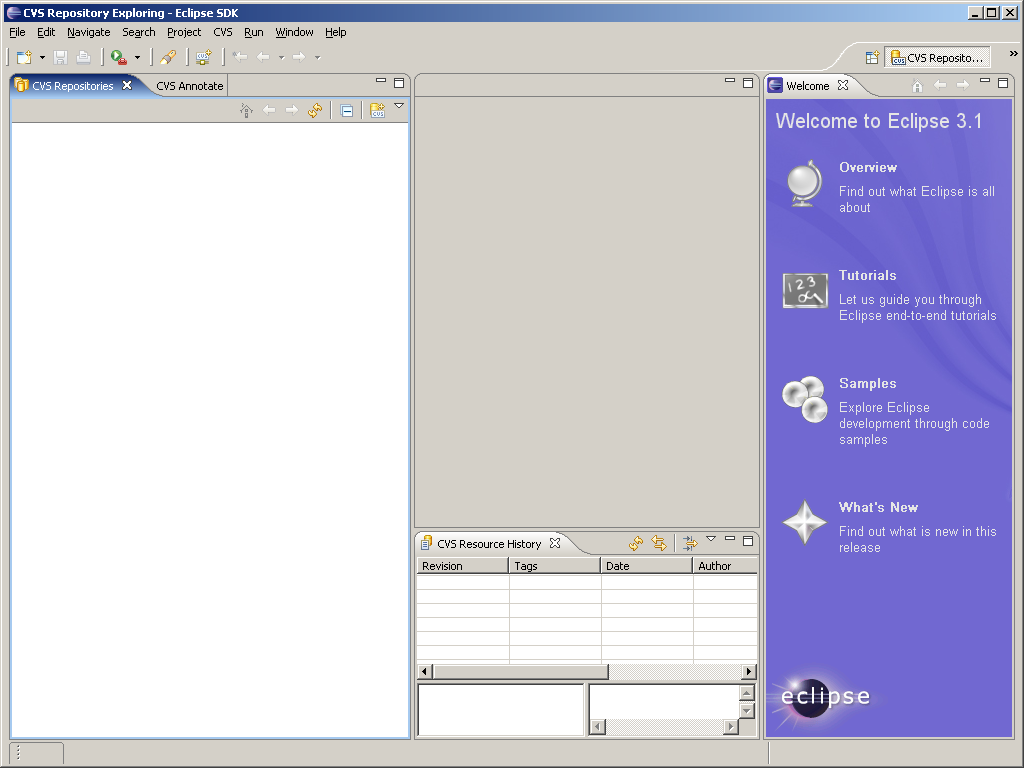
\includegraphics[scale=.33]{image/eclipse-cvs-1}
  \caption{CVS Exploring Perspective}\label{fig:eclipse-cvs-1}
\end{figure}

To add a new repository location press the left mouse button on this
tab and select \menu{New \sub Repository Location\ldots} (see
figure~\ref{fig:eclipse-new-repository}). This brings up the dialog
shown in figure~\ref{fig:eclipse-add-cvs}. Here you can enter the
coordinates of the \ExTeX\ CVS repository.
\begin{figure}[htp]
  \hbox{}\hfill
  \subfigure[New Repository Location\label{fig:eclipse-new-repository}]{%
    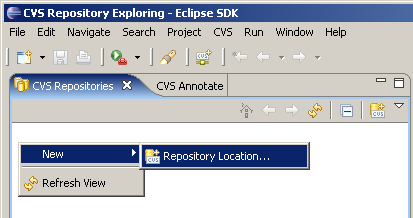
\includegraphics[scale=.4]{image/eclipse-new-repository}}%
  \hfill
  \subfigure[The Coordinates of the \ExTeX\ CVS
  Repository\label{fig:eclipse-add-cvs}]{%
    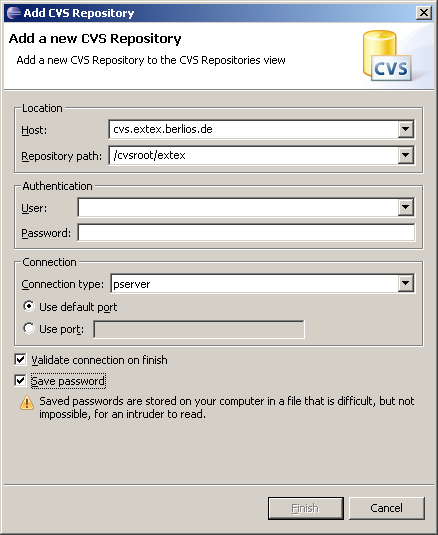
\includegraphics[scale=.4]{image/eclipse-add-cvs}}%
  \caption{Adding the \ExTeX\ CVS Repository}
\end{figure}

Note that you have to enter your account at Berlios and its password
into the appropriate fields. If you do not have an account you can use
the account name \texttt{anonymous} without any password to get
reading access to the sources.

For this step you need online access to the internet. When the form is
submitted with the OK button, the accessibility of the repository
location is checked. Upon success the new repository location is
added to the list of repository locations as can be seen in
figure~\ref{fig:eclipse-cvs}.
\begin{figure}[htbp]
  \hbox{}\hfill
  \subfigure[The \ExTeX\ Repository Listed\label{fig:eclipse-cvs}]{%
    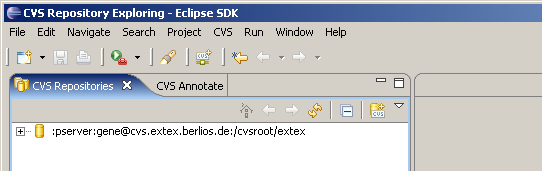
\includegraphics[scale=.4]{image/eclipse-cvs}}%
  \hfill
  \subfigure[Selecting to check-out of
  \ExTeX\label{fig:eclipse-checkout-extex}]{%
    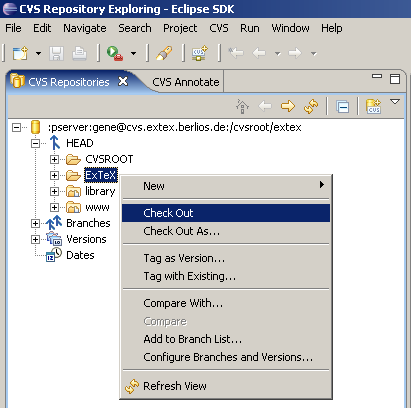
\includegraphics[scale=.4]{image/eclipse-checkout-extex}}%
  \caption{Checking-out of \ExTeX}
\end{figure}

The next step consists of the check-out of the sources into an Eclipse
project. To accomplish this you have to open the repository location
and the HEAD within. Right-click the item \texttt{ExTeX} in the list
(see figure~\ref{fig:eclipse-cvs}) and select \menu{Checkout} in the
appearing context menu (see figure~\ref{fig:eclipse-checkout-extex}).
This will instruct Exclipe to create a new project in the workspace
and fill it with the files from the repository.

Eclipse shows a progress bar during the check-out (see
figure~ref{fig:eclipse-checkout}). This operation may take some time
-- we have been really busy creating files. When the checkout is
finished you will find the project \texttt{ExTeX} in Eclipse
containing the files within. The appearance of the Package View with
those files is shown in figure~\ref{fig:eclipse-extex-project}.
\begin{figure}[htp]
  \hbox{}\hfill
  \subfigure[The Checkout Progress Bar\label{fig:eclipse-checkout}]{%
    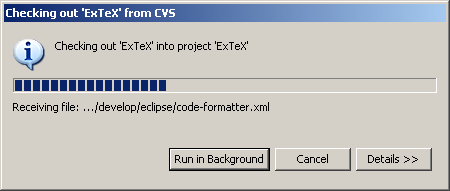
\includegraphics[scale=.4]{image/eclipse-checkout}}%
  \hfill
  \subfigure[The \ExTeX\ Project in the Package
  View\label{fig:eclipse-extex-project}]{%
    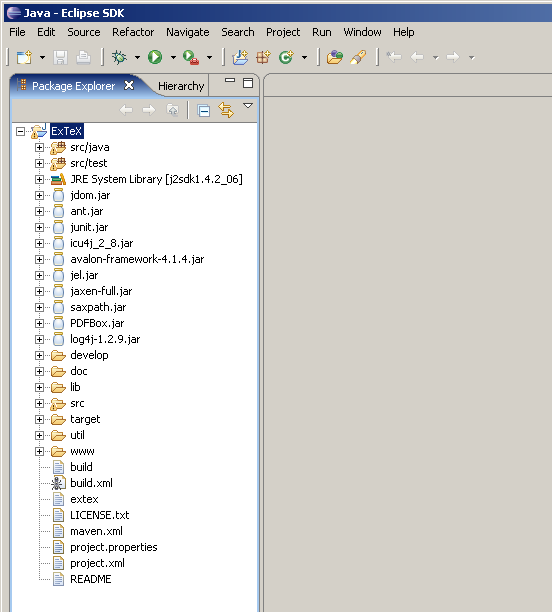
\includegraphics[scale=.4]{image/eclipse-extex-project}}%
  \caption{Checking out \ExTeX\ from the Repository}
\end{figure}

\subsection{Configuring Eclipse}

Eclipse can be configured in a wide range. In the following sections
some configuration options are proposed for the seamless development
of \ExTeX. The configuration is performed via the preferences dialog.
This dialog can be opened via \menu{Window \sub Preferences\ldots}
\begin{figure}[htp]
  \hbox{}\hfill
  \subfigure[Eclipse Preferences\label{fig:eclipse-preferences}]{%
    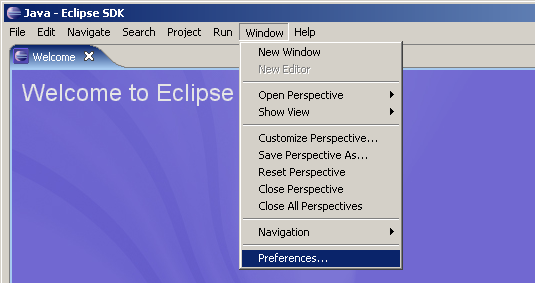
\includegraphics[scale=.4]{image/eclipse-preferences}}%
  \hfill
  \subfigure[Eclipse Print Margin\label{fig:eclipse-print-margin}]{%
    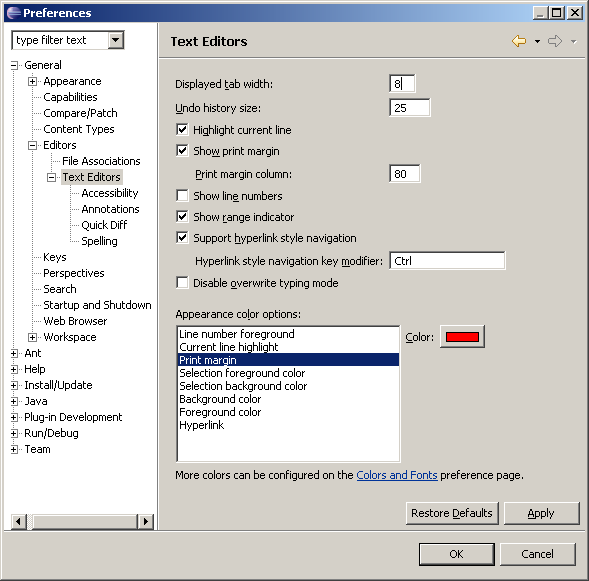
\includegraphics[scale=.4]{image/eclipse-print-margin}}%
  \caption{Some simple Settings}
\end{figure}

This menu brings up a dialog with many tabs which can be used to
adjust the behaviour of Eclipse in many ways. The first step described
below consists of the adaption of the appearance of the text editors.
In the tree view on the left side of the dialog select \menu{General
  \sub Editors \sub Text Editors} as shown in
figure~\ref{fig:eclipse-print-margin}.

Now you can adjust some values on the right side of the dialog. Set
the tag width to 8. Check the item \menu{Show print margin}. Adjust
the print margin to 80. And finally change the print color to red. The
settings are stored in the workspace by accepting the settings with
the \menu{OK} button.

The rational is that the tabs should be used in the traditional sense
of eight chracters wide. In fact this is just a fallback. Usually tabs
should be avoided where possible. The print margin of 80 is a weak
rule. Try to limit yourself to this width. Sometimes it is not
reasonable. Thus the checkstyle rules allow some more characters
before complaining.

The following sections describe some more of the configuration
options. You should really consider to follow the instructions to make
maximal use of the configurations provided with \ExTeX.



\subsection{Code Templates}

Code templates provide a convenient way of filling in a frame for the
documentation whenever some code is generated by Eclipse. The \ExTeX\
repository contains in the file
\File{develop/eclipse/codetemplates.xml} some definitions of code
templates. To import those definitions use the preferences (see
figure~\ref{fig:eclipse-preferences}). Here select the item \menu{Java
  \sub Code Style \sub Code Templates}. The button \menu{Import\ldots}
can leads to a file selector where the file
\File{develop/eclipse/codetemplates.xml} should be entered.
\begin{figure}[htp]
  \centering  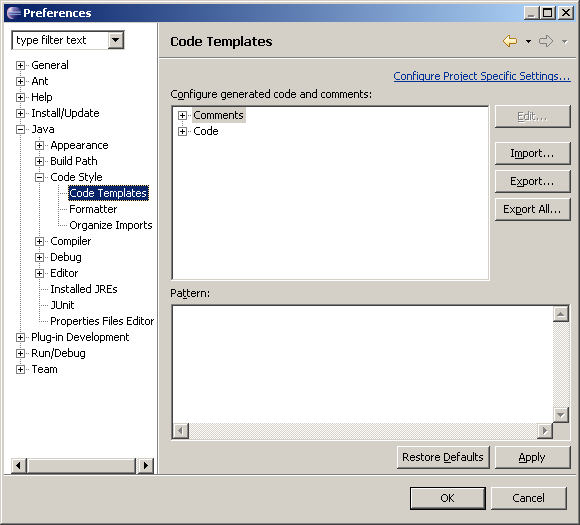
\includegraphics[scale=.4]{image/eclipse-templates}
  \caption{Eclipse Preferences}\label{fig:eclipse-templates}
\end{figure}

After the code templates have been loaded a minor adaption is
required. The entry under the key \menu{Comments \sub Types} containes
hard-wired a name and email address of the author. Here the own name
and email address should be entered (see figure~{fig:eclipse-template-author}).
\begin{figure}[htp]
  \centering  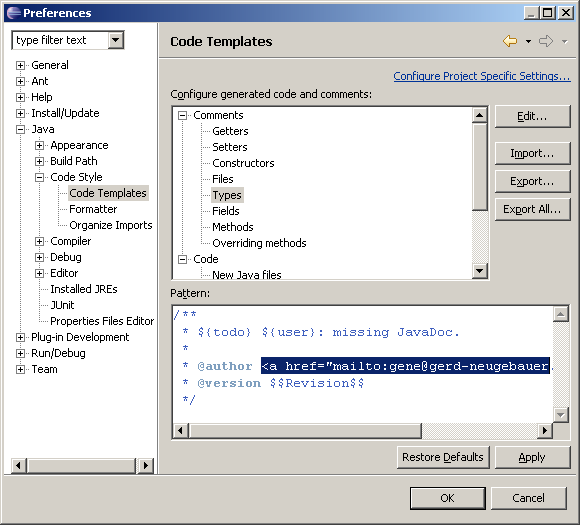
\includegraphics[scale=.4]{image/eclipse-template-author}
  \caption{Code Template Author Name}\label{fig:eclipse-template-author}
\end{figure}


\subsection{The Code Formatter}

Eclipse comes has a code formatter which can be invoked easily. This
code formatter can be configured for different needs. A configuration
for \ExTeX\ is contained in the repository under
\texttt{develop/eclipse/formatter.xml}. In Eclipse the preference page
can be found under the key \menu{Java \sub Code Style \sub Formatter}.
ere you can use the button \menu{Import\dots} and select the
configuration file. Now the profile ``gene'' is loaded and can be
selected. This is shown in figure~\ref{fig:eclipse-formatter-gene}.
\begin{figure}[htp]
  \centering  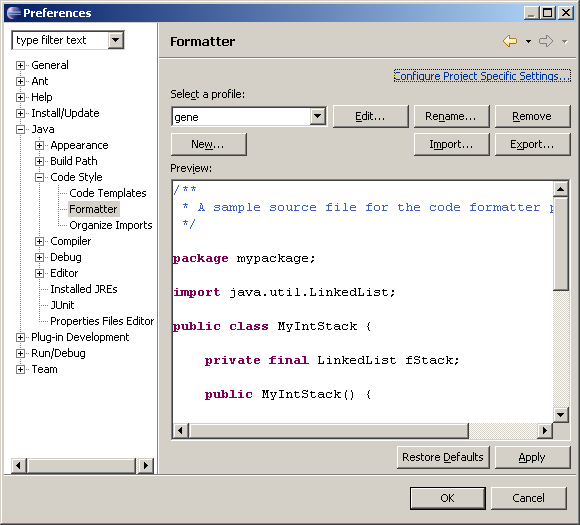
\includegraphics[scale=.4]{image/eclipse-formatter-gene}
  \caption{Settings for the Code Formatter}\label{fig:eclipse-formatter-gene}
\end{figure}


The formatter for Ant files has distinct parameters which should be
adapted. The Prference page can be found under the key \menu{Ant \sub
  Editor \sub Formatter}. The values should be adjusted as shown in
figure~\ref{fig:eclipse-ant-formatter}.
\begin{figure}[htp]
  \centering  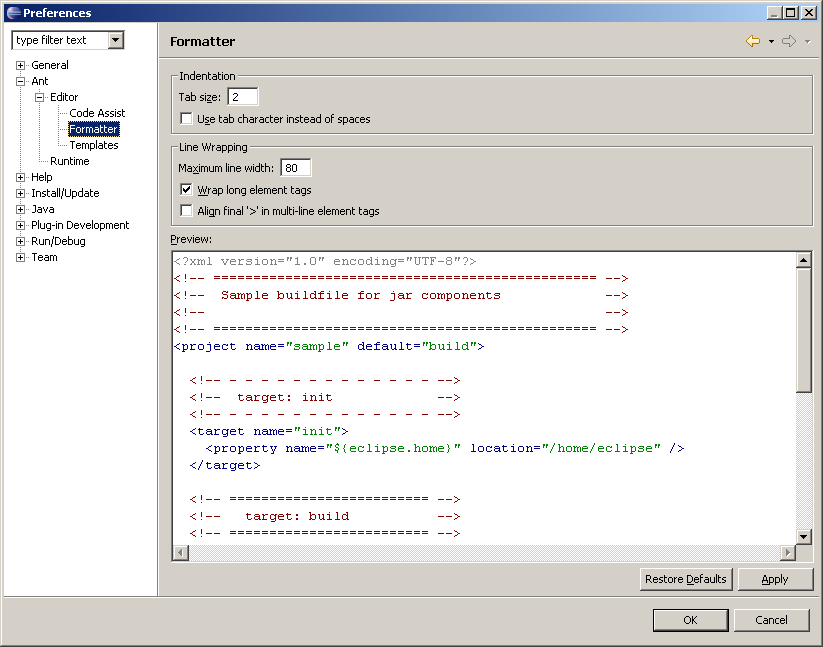
\includegraphics[scale=.4]{image/eclipse-ant-formatter}
  \caption{Settings for the Ant Formatter}\label{fig:eclipse-ant-formatter}
\end{figure}


\subsection{Checkstyle}

Checkstyle is a tool for checking the adherence of Java source code to
certain rules. The rules can be freely configured. The \ExTeX\
repository contains a set of rules for checkstyle.

Checkstyle comes in a command line version and as a plug-in for
Eclipse. This plugin has to be installed first.

\subsubsection*{Install Checkstyle plugin}

To install the checkstyle plugin over the update wizard, use
\menu{Help \sub Software Update \sub Find and Install \sub
Search for new features to install \sub Next \sub New Remote Site } and input the name
'checkstyle' and the URL \url{http://eclipse-cs.sourceforge.net/update}
(see figure~\ref{fig:eclipse-checkstyle-url}).
\begin{figure}[htp]
  \centering  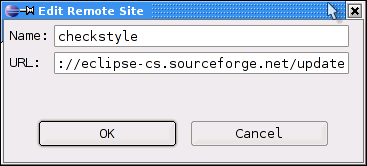
\includegraphics[scale=.5]{image/eclipse-checkstyle-url}
  \caption{Checkstyle URL}\label{fig:eclipse-checkstyle-url}
\end{figure}

\subsubsection*{Configure Checkstyle}

To set the configuration use \menu{Window \sub Preferences \sub Checkstyle }.
Create a new configuration and set the values in
figure~\ref{fig:eclipse-checkstyle-config}.

The configuration is stored in \File{develop/eclipse/extex\_checkstyle.xml}.

\begin{figure}[htp]
  \centering  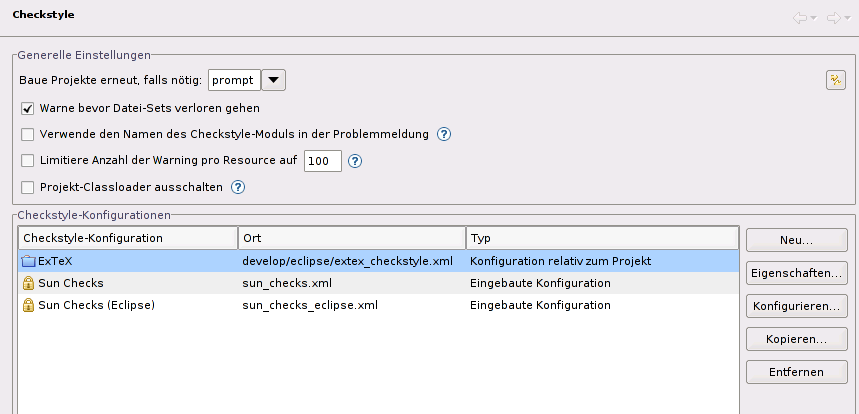
\includegraphics[scale=.5]{image/eclipse-checkstyle-config}
  \caption{Checkstyle configuration}\label{fig:eclipse-checkstyle-config}
\end{figure}

\subsubsection*{Enable Checkstyle}

To enable the checks set in \menu{Project \sub Properties \sub Chekcstyle}
the configuration to \emph{ExTeX} (see figure~\ref{fig:eclipse-checkstyle-enable}).
\begin{figure}[htp]
  \centering  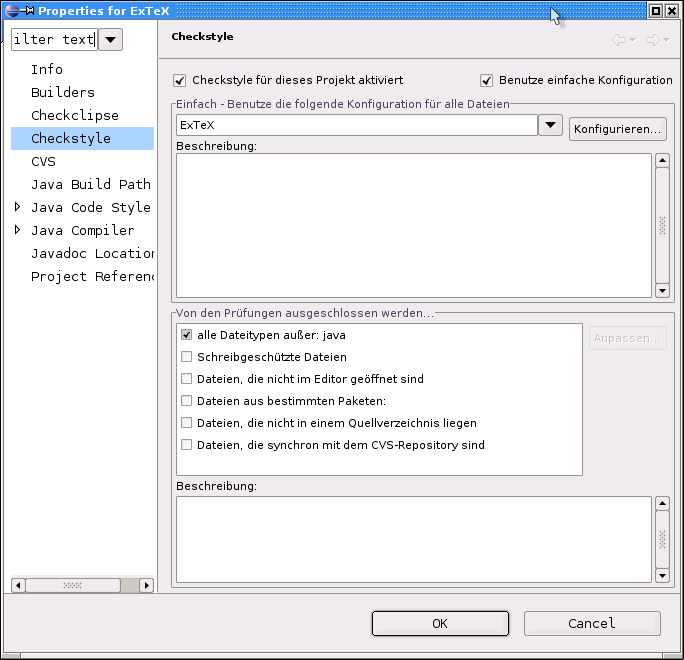
\includegraphics[scale=.5]{image/eclipse-checkstyle-enable}
  \caption{enable Checkstyle}\label{fig:eclipse-checkstyle-enable}
\end{figure}


\subsection{Spelling}

Since English is not the native language of each developer it is a
good idea to enable the spell checking of the source code. This
feature is provided by Eclipse. In figure~ref{fig:eclipse-spelling}
you can seen the preference page where you can activate the spell
checking and provide a dictionary.
\begin{figure}[htp]
  \centering
  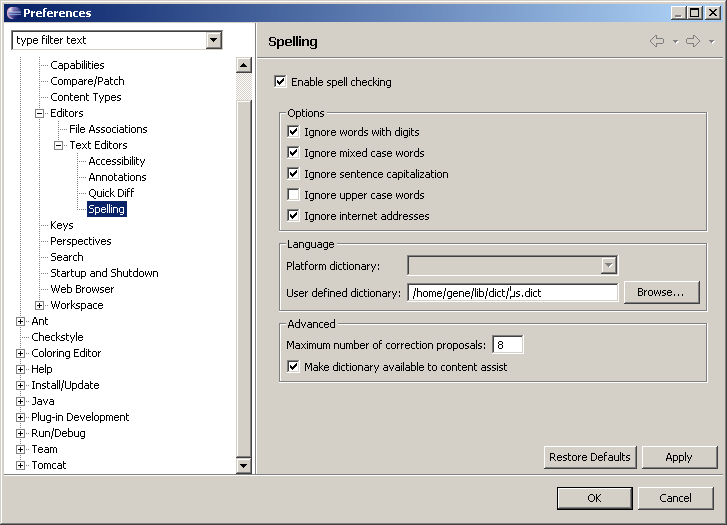
\includegraphics[scale=.4]{image/spelling}
  \caption{Spelling Preferences}\label{fig:eclipse-spelling}
\end{figure}

A dictionary can be got from SCOWL
(\url{http://wordlist.sourceforge.net/}). You might want to use the US
dictionary of medium size. Since this contains enough words to fit but
not too much obscure words which hide typos.

After the spell checking is activated potential typos are marked in
the editor with yellow lines. Correction proposals can be requested
with the quick fix shortcut Ctrl-1.


\subsection{Compiling \ExTeX}

Any source file in Eclipse is compiled automatically when the file is
saved. Thus it is usually not necessary to compile things manually. If
you feel the need to recompile everything you can achieve this by
selecting \menu{Project \sub Clean\ldots} while the item \menu{Project
  \sub Build Automatically} is checked (see
figure~\ref{fig:eclipse-recompile}).
\begin{figure}[thp]
  \centering
  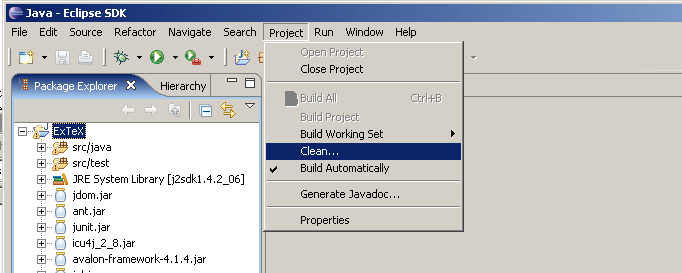
\includegraphics[scale=.4]{image/eclipse-recompile}
  \caption{Recompiling a Project}\label{fig:eclipse-recompile}
\end{figure}

Another recompilation can be triggered via the Ant task \texttt{compile}.

\subsection{Running \ExTeX}

\ExTeX\ can be run from within Eclipse. We will describe here the
execution of the compiled sources from a workspace. The executio of an
external program would be an alterative. But this is only of minor
relevance for a developer.

To run \ExTeX\ on some input file you have to create a run profile.
The profile is kept and can be used the next time again. To create a
run profile select the toolbar item \menu{Run\dots} in the Java
perspective (see figure~\ref{fig:eclipse-run-menu}). In the appearing
dialog select \menu{Java Application} and press the button \menu{New}.
Now you can fill in the tabs as seen in figure~\ref{fig:eclipse-run}.
Enter a name, the project and the main class. The main class to use is
\texttt{de.dante.extex.main.TeX}.
\begin{figure}[htp]
  \hbox{}\hfill
  \subfigure[The Run Menu\label{fig:eclipse-run-menu}]{%
    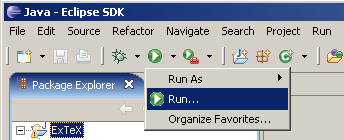
\includegraphics[scale=.4]{image/eclipse-run-menu}}%
  \hfill
  \subfigure[Creating a run configuration\label{fig:eclipse-run}]{%
    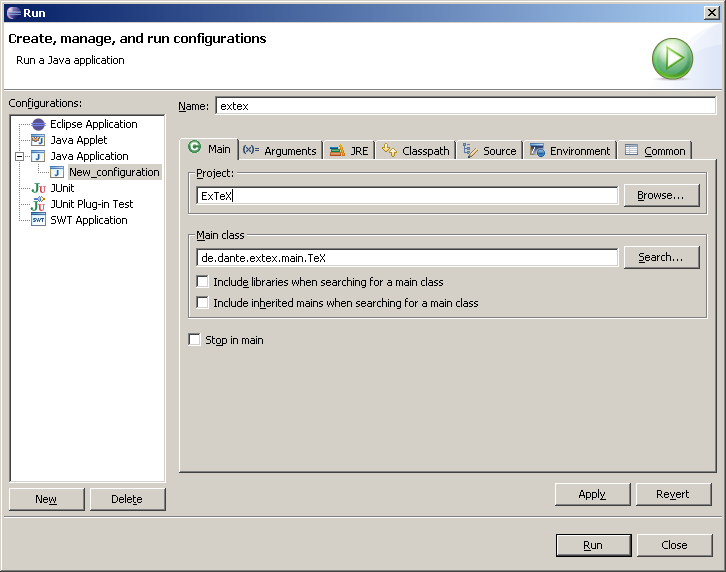
\includegraphics[scale=.4]{image/eclipse-run}}%
  \caption{Checking out \ExTeX\ from the Repository}
\end{figure}

On the Arguments tab you can enter the arguments for the invocation of
\ExTeX. These are the same arguments which can also be used on the
command line. Usually here the input file is given (see
figure~\ref{fig:eclipse-run-args}.
\begin{figure}[thp]
  \centering
  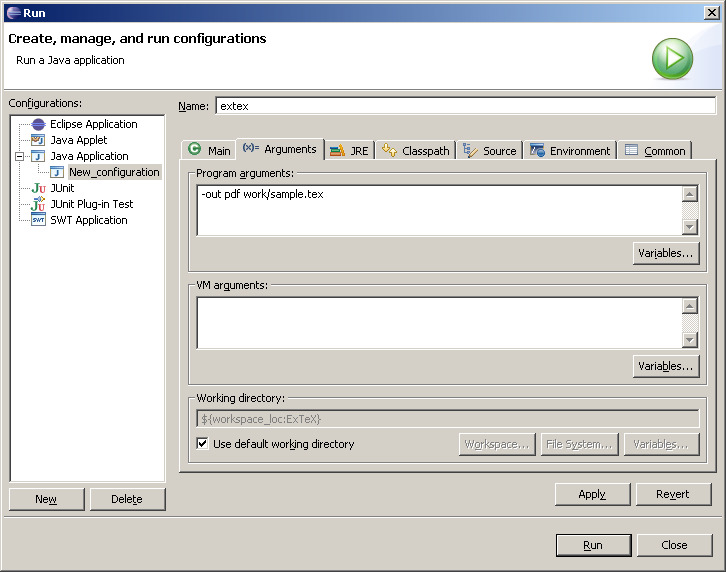
\includegraphics[scale=.4]{image/eclipse-run-args}
  \caption{Arguments for Running \ExTeX}\label{fig:eclipse-run-args}
\end{figure}

The \menu{Run} button submits the command. A Console view is opened
which can be used to interact with the the program -- like in the
command line interpreter.


\subsection{Committing Changes}

Eclipse ships with a CVS plugin which hides the details of the
underlying version control system. Thus things are quite simple for
the newcomers. On the other hand they are differnt from the procedure
on the command line or other tools whic mimic the command line (like
WinCVS or TortoiseCVS).

The metaphor used in Eclipse is the synchronisation of the workspace
with the reporsitory. In the course of this syncronisation changes in
the workspace files are committed to the repository, changes from the
repository are updated into the workspace, and conflicts can be
resolved. The conflict resolution -- also known as merging -- is the
demanding task. Thus it has to be performed by a human.

To start the synchronisation select in the \menu{Package Manager} or
\menu{Navigator} view the topmost \ExTeX\ node and activate in the
context menu (right mouse button) the entry \menu{Team \sub Synchronize
with Repository} (see figure~\ref{fig:eclipse-team}).
\begin{figure}[htp]
  \centering
  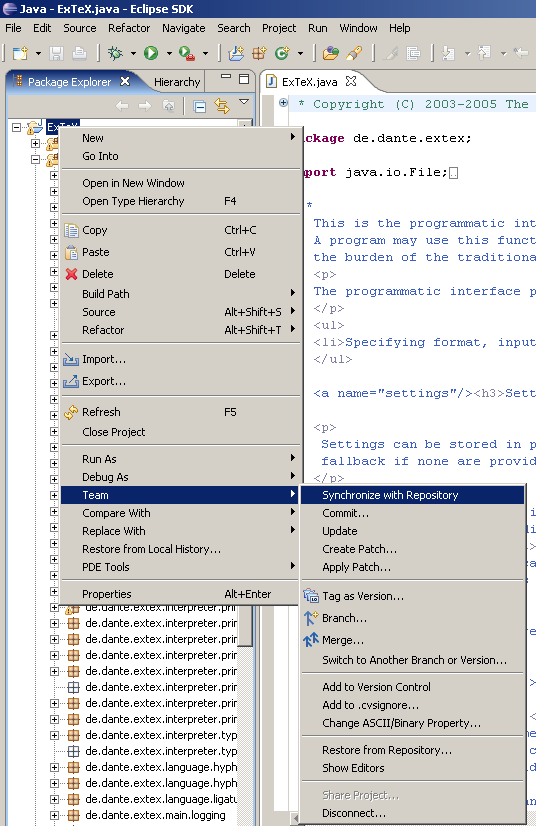
\includegraphics[scale=.4]{image/eclipse-team}
  \caption{Starting Synchronization}\label{fig:eclipse-team}
\end{figure}



\INCOMPLETE



\subsection{Running Ant from within Eclipse}\label{sec:eclipse.ant}

To use Ant from within Eclipse you have to open the Ant view. This can
be acomplished via the menu \menu{Window \sub Show View \sub Ant} (see
figure~\ref{fig:eclipse-ant-open}).

In this view use the leftmost tool to add an Ant file. In the file
selector choose the file \File{ExTeX/build.xml}. The Ant file is added
to the (previously empty) list. It can be open to show the Ant target
available (see figure~\ref{fig:eclipse-ant}).
\begin{figure}[htp]
  \hbox{}\hfill
  \subfigure[Opening an Ant View\label{fig:eclipse-ant-open}]{%
    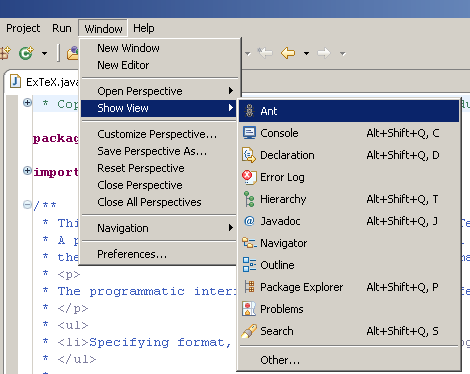
\includegraphics[scale=.4]{image/eclipse-ant-open}}%
  \hfill
  \subfigure[The Ant View for \ExTeX\label{fig:eclipse-ant}]{%
    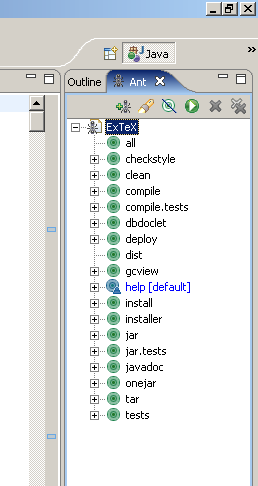
\includegraphics[scale=.4]{image/eclipse-ant}}%
  \caption{Ant in Eclipse}
\end{figure}

A double click on a target starts it's execution. The output is shown
in a Console view.

A description of the targets can be found in section~\ref{sec:Ant}.


\subsection{Creating Javadoc}

To create the Javadoc HTML description of the sources you can use the
Ant target \texttt{javadoc}. See sections \ref{sec:eclipse.ant} and
\ref{sec:Ant}. The result can be found in the directory
\File{target/javadoc}.


\subsection{Creating the Installer}

To create the inastaller you can use the Ant target
\texttt{installer}. See sections \ref{sec:eclipse.ant} and
\ref{sec:Ant}. The result can be found in the file
\File{target/ExTeX-setup.jar}.


